\documentclass[10pt,a4paper]{article}

\usepackage{orcidlink}
\usepackage[a4paper,margin=2.5cm]{geometry}
\usepackage[T1]{fontenc}
\usepackage[utf8]{inputenc}
\usepackage{lmodern}
\usepackage{microtype}
\usepackage{amsmath,amssymb,mathtools}
\usepackage{seqsplit, stmaryrd}
\usepackage{booktabs}
\usepackage{graphicx}
\usepackage{float}
\usepackage{caption}
\usepackage{subcaption}
\usepackage{enumitem}
\usepackage[table]{xcolor}
\usepackage{listings}
\usepackage{hyperref}

\hypersetup{
    colorlinks=true,
    linkcolor=blue,
    citecolor=blue,
    urlcolor=blue
}

\lstset{
    basicstyle=\ttfamily\small,
    breaklines=true,
    frame=single,
    numbers=left,
    numberstyle=\tiny,
    showstringspaces=false
}

\title{
    \textbf{2IMF25 Automated Reasoning}\\
    \large Practical Assignment
}

\author{
    Tygo van den Hurk \orcidlink{0009-0003-4182-5076} (1705709) \\
    \texttt{t.j.f.h.v.d.hurk@student.tue.nl}
    \and
    Bram Boomen (???????) \\
    \texttt{b.boomen@student.tue.nl}
    \and
    Librecht Kuijvenhoven (2204975) \\
    \texttt{l.kuijvenhoven@student.tue.nl}
}

\date{
    Group: 66\\
    \today
}

\renewcommand{\geq}{\geqslant}
\renewcommand{\leq}{\leqslant}
\renewcommand{\ge}{\geqslant}
\renewcommand{\le}{\leqslant}

\begin{document}
    \maketitle

    \begin{abstract}
        In this course, we study a number of techniques and algorithms,
        including satisfiability for propositional (Boolean) logic,
        satisfiability modulo theories (SMT), binary decision diagrams (BDDs),
        model checking, and first-order logic. The course covers both the
        underlying algorithms and solving real-world problems using the tools
        that implement those algorithms.
    \end{abstract}

    \newcommand{\Dupples}{\texttt{Dupples}}
\newcommand{\Nuzzles}{\texttt{Nuzzles}}
\newcommand{\Prittles}{\texttt{Prittles}}
\newcommand{\Skipples}{\texttt{Skipples}}
\newcommand{\Crottles}{\texttt{Crottles}}

\section{Exercise 1}

    \subsection{Approach}

        I started out by modeling the products first, so I made an enum and
        gave it properties such as name, weight, and required amount. Then
        all I had to do was iterate over them and creating variables using
        the weight and the required amount for each product.

        Next, I started with the trucks. Trucks have a maximum weight they can
        carry, plus an amount for each product they're carrying. So I added
        those two fields and made the variables for: the total weight in the
        truck, the amount of product $p_1$, the amount for product $p_2$, ...
        
        To finish the trucks off I just had to assert that the weight is
        between 0 and the max capacity, and that it is equal to the sum of
        the weights of the products being transported. And finally the amount
        of products being transported had to be less the 10.

        The last part was just asserting a couple more global constraints. Like
        how the total amount of a product being transported is the same as the
        sum of what the trucks are transporting.

    \subsection{Implementation}

        \subsubsection{constants}
            \begin{itemize}
                \item
                    The amount of trucks as
                    $\texttt{amount\_of\_trucks} = 6$
                \item 
                    The maximum load capacity per truck in kg
                    $\texttt{max\_weight\_truck} = 8000$
                \item
                    The maximum amount of products in a truck
                    $\texttt{max\_amount\_truck} = 10$
            \end{itemize}

        \subsubsection{Variables}
            \begin{itemize}
                \item
                    $\alpha_{p,t} \in \mathbb{Z}$ representing the total amount
                    of a product $p$ being transported in a truck $t$.
                \item
                    $\beta_{p} \in \mathbb{Z}$ representing the total amount of
                    a product $p$ being transported.
                \item
                    $\gamma_{t} \in \mathbb{Z}$ representing the total weight a
                    truck $t$ is transporting.
            \end{itemize}

        \subsubsection{Sets}
            \begin{itemize}
                \item 
                    The set of products: $P = \big\{
                        \Dupples,
                        \Nuzzles,
                        \Prittles,
                        \Skipples,
                        \Crottles
                    \big\}$.
                \item 
                    The set of products that have a required amount: 
                    $P_r = P \setminus \{ \Dupples \}$
                \item
                    The set of trucks: $T = \big\{
                        1, 2, ..., \texttt{amount\_of\_trucks}
                    \big\}$
                \item
                    The set of trucks that can transport \Skipples:
                    $T_s = \big\{ 1, 2 \big\}$
            \end{itemize}

        \subsubsection{Functions}        
            \begin{itemize}
                \item 
                    A function to get the required amount of a product:
                    \[
                        r : P_r \to \mathbb{N},\qquad r(p) = \begin{cases}
                            6  & \text{if } p = Nuzzles  \\
                            12 & \text{if } p = Prittles \\
                            15 & \text{if } p = Skipples \\
                            8  & \text{if } p = Crottles
                        \end{cases}
                    \]
                \item 
                    A function to get the weight per product:
                    \[
                        w : P \to \mathbb{N},\qquad w(p) = \begin{cases}
                            800  & \text{if } p = Nuzzles  \\
                            405  & \text{if } p = Prittles \\
                            500  & \text{if } p = Skipples \\
                            2500 & \text{if } p = Crottles \\
                            600  & \text{if } p = Dupples \\
                        \end{cases}
                    \]
            \end{itemize}
        
        \subsubsection{Assertions}
            For the total amount of product $p$ being transported I created the
            following formulas:

            \begin{itemize}
                \item 
                    Asserting that the amount of products being transported are
                    non-negative:
                    \[
                        \bigg(
                            \bigwedge_{(p, t) \in P \times T} 
                                \alpha_{p,t} \ge 0
                        \bigg) \wedge \bigg(
                            \bigwedge_{p \in P} \beta_p \ge 0
                        \bigg)
                    \]
                \item
                    Asserting that the required amount is transported:
                    \[
                        \bigwedge_{p \in P_r} \beta_{p} = r(p)
                    \]
                \item
                    Asserting that the weight of a truck is the sum of its
                    products, and is in a valid range:
                    \[
                        \bigwedge_{t \in T} 0 \leq \gamma_{t} = \bigg(
                            \sum_{p \in P} \Big(
                                \alpha_{p,t}\cdot w(p)
                            \Big)
                        \bigg) \leq \texttt{max\_weight\_truck}
                    \]
                \item
                    asserting a truck $t$ transports at most 10 items:
                    \[
                        \bigwedge_{t \in T} \bigg(
                            \sum_{p \in P} \alpha_{p,t}
                        \bigg) \leq 10
                    \]
                \item
                    asserting that only some trucks can transport
                    \texttt{Skipples}:
                    \[
                        \bigwedge_{t \in T} \bigg(
                            \big(
                                t \not\in T_s 
                            \big) \implies \big(
                                \alpha_{p,t} = 0
                            \big)
                        \bigg) \qquad \text{ where $p$ = \Skipples}
                    \]
                \item
                    asserting the total amount of a product $p$ being
                    transported is the sum of what the trucks are transporting:
                    \[
                        \bigwedge_{p \in P} \bigg(
                            \beta_p = \Big( \sum_{t \in T} \alpha_{p,t}
                            \Big)
                        \bigg)
                    \]
                \item 
                    asserting that \Prittles\text{ } are spread over at least
                    5 trucks:
                    \[
                        \sum_{t \in T} \bigg(
                            \operatorname{ite}\Big(
                                \big(\alpha_{p,t} > 0\big),\ 1,\ 0
                            \Big)
                        \bigg) \geq 5 \qquad \text{ where p = \Prittles}
                    \]
            \end{itemize}

            \noindent The goal is of course to maximise the amount of \Dupples:
            
            \[
                \text{maximize } \beta_p \text{ where $p = \Dupples$}
            \]

            \noindent For question b there was one more asserting we have to
            make. Namely, \Crottles cannot be transported without at least 2
            \Dupples\text{ } in the same truck:

            \[
                \bigwedge_{t \in T} \bigg(
                    \Big(
                        \alpha_{p_1,t} > 0
                    \Big) \implies \Big(
                        \alpha_{p_2,t} \geq 2
                    \Big)
                \bigg) \qquad 
                    \text{ where $p_1 = \Crottles$}
                    \text{ and $p_2 = \Dupples$}
            \]

            \noindent I did leave out all mentions of truck speed. I did this
            on purpose as the driving speed does not affect the amount of
            \Dupples\text{ } I can deliver and that would just slow the solver
            down, and make it harder to implement.

    \subsection{Results}

        The results were that both sub-questions were satisfiable. I've created
        tables to help visualize the results.

        \subsubsection{Visualisation Exercise 1a}

            \begin{table}[ht]
                \centering
                \caption{Distribution of products over the trucks for 1a.}
                \label{tab:exercise1a}
                \begin{tabular}{c|ccccc|c}
                    \textbf{Truck} & \textbf{Nuzzles} & \textbf{Prittles} & 
                    \textbf{Skipples} & \textbf{Crottles} & \textbf{Dupples} &
                    \textbf{Weight (kg)} \\
                    \hline
                    %%% T | N | P | S | C | D | W
                        1 & 0 & 1 & 6 & 1 & 2 & 7105 \\
                        2 & 0 & 0 & 9 & 1 & 0 & 7000 \\
                        3 & 2 & 2 & 0 & 1 & 5 & 7910 \\
                        4 & 0 & 1 & 0 & 2 & 4 & 7805 \\
                        5 & 4 & 4 & 0 & 1 & 1 & 7920 \\
                        6 & 0 & 4 & 0 & 2 & 2 & 7820 \\
                    \hline
                    \textbf{Total} & \textbf{6} & \textbf{12} & \textbf{15} &
                    \textbf{8} & \textbf{14} & \\
                \end{tabular}
            \end{table}

        \subsubsection{Visualisation Exercise 1b}

            \begin{table}[ht]
                \centering
                \caption{Distribution of products over the trucks for 1b.}
                \label{tab:exercise1b}
                \begin{tabular}{c|ccccc|c}
                    \textbf{Truck} & \textbf{Nuzzles} & \textbf{Prittles} & 
                    \textbf{Skipples} & \textbf{Crottles} & \textbf{Dupples} &
                    \textbf{Weight (kg)} \\
                    \hline
                    %%% T | N | P | S | C | D | W
                        1 & 0 & 1 & 6 & 1 & 2 & 7105 \\
                        2 & 1 & 0 & 9 & 0 & 0 & 5300 \\
                        3 & 0 & 4 & 0 & 2 & 2 & 7820 \\
                        4 & 3 & 3 & 0 & 1 & 3 & 7915 \\
                        5 & 1 & 2 & 0 & 2 & 2 & 7810 \\
                        6 & 1 & 2 & 0 & 2 & 2 & 7810 \\
                    \hline
                    \textbf{Total} & \textbf{6} & \textbf{12} & \textbf{15} &
                    \textbf{8} & \textbf{11} & \\
                \end{tabular}
            \end{table}

    \section{Problem 2: PCB Layout}
The goal of this exercise is to place 14 different chips on two PCB
boards, without the chips overlapping with another chip, battery, or
camera. However, certain chips are prone to overheating and cannot be
placed near each other. Keeping these constraints in mind, is it
possible to find a valid placement of the chips for 3 different PCB
designs?

    \subsection{Solution}
            
        \subsubsection{Constants}
            \begin{itemize}
                \item $n=14$, the number of chips that need to be placed
                \item $m = 3$, the number of objects on the PCB
            \end{itemize}

            \begin{table}[h]
                \centering
                \begin{tabular}{l|cccccccccccccc}
                \toprule
                \multicolumn{15}{c}{Chips} \\
                \midrule
                width & 5 & 5 & 4 & 4  & 5 & 3 & 7 & 6  & 6  & 4  & 6 & 5  & 6  & 5  \\
                height& 6 & 6 & 6 & 10 & 7 & 7 & 7 & 10 & 12 & 10 & 9 & 11 & 10 & 10 \\
                hot?  & \checkmark & \checkmark & & & & \checkmark & & & & & & & &   \\
                \bottomrule
                \end{tabular}
            \end{table}

            It is possible for the PCB's to contain objects like batteries or 
            camera's, just like the different chip sizes these objects are part of
            the PCB design that are already determined by the problem description.

            \begin{table}[h]
                \centering
                \begin{tabular}{l|cccccc}
                \toprule
                \multicolumn{6}{c}{Objects} \\
                \midrule
                label      & Battery & Battery & Camera A & Camera B  & Camera C \\
                width      & 12 & 14 & 7 & 11  & 15 \\
                height     & 8 & 12 & 5 & 5 & 5 \\
                x position & 0 & 0 & 17 & 13 & 9 \\
                y position & 0 & 0 & 22 & 22 & 22 \\
                PCB        & 1 & 2 & 2 & 2  & 2 \\
                \bottomrule
                \end{tabular}
            \end{table}

    \subsection{Variables}

        We use different parameters for the problem:
        
        \begin{itemize}
            \item $n=$ the number of chips that need to be placed
            \item $m = $ the number of objects on the PCB
        \end{itemize}

        For $i \in \{0, 1, ..., n-1\}$, we have the following variables:
        \begin{itemize}
            \item $X_i$ representing the $x$ coordinate of the lower left corner
                of chip $i$.
            \item $Y_i$ representing the $y$ coordinate of the lower left corner
                of chip $i$.
            \item $R_i$ representing whether a a chip $i$ is rotated.
            \item $W_i$ representing the width of the chip $i$.
            \item $H_i$ representing the height of chip $i$.
            \item $PCB_i$ representing the PCB where chip $i$ is placed on.
            \item $Hot_i$ representing whether chip $i$ becomes warm under load.
        \end{itemize}

        We further expand on these variables by defining values for the $x$ and
        $y$ intervals, these will aid us in detecting overlaps:
        
        $$X_i^{min} = X_i$$

        $$
        X^{\max}_{i} = \begin{cases} 
            X_i + W_i & \text{if } R_i = 0, \\
            X_i + H_i & \text{otherwise}
        \end{cases}
        $$

        Repeat the same procedure for $Y^{min}_i$ and $Y^{max}_{i}$

        Lastly we use these properties not only for the chips but also for the
        objects that can be placed upon the PCB like the battery or camera's.
        For a range $i \in \{0, ..., m-1\}$, we define the variables as
        follows, $X_i^o$, $Y_i^o$, $R_i^o$, $W_i^o$, $H_i^o$, but defined with
        the superscript $o$, to differentiate between the chip related
        variables.

        To build up the CNF which will solve the PCB layout problem we use the
        variables mentioned above, to construct the following placement
        constraints:

        \begin{itemize}
            \item Chips cannot overlap
            \item Chips should be placed on the PCB
            \item Chips cannot overlap with Objects
            \item Chips that produce heat cannot be placed near each other.
        \end{itemize}

    \subsection{Constraints}
        
        \subsubsection{Chip Overlap}

            \begin{itemize}
                \item Overlap constraint:
                    \[
                        \bigwedge_{i=0}^{n}\bigwedge_{j=0}^{n} \lnot Overlap(i, j)
                    \]

                    $Chip_i$ and $Chip_j$ overlap only if they overlap in the
                    x-intervals, y-intervals and are placed on the same PCB.
                    
                    \[  
                        Overlap(i,j) = 
                        Overlap_x(i, j) \land
                        Overlap_y(i, j) \land
                        PCB[i] = PCB[j]
                    \]

                    We check for overlap on the x-interval with the following
                    equation:

                    \[
                        Overlap(i, j) : 
                        x_i^{min} < x_j^{max} \land x_i^{min} < x_j^{max}
                    \]
                    
                    Repeat the process for the y direction.

            \end{itemize}

            $$
            \begin{aligned}
                & (R[j] = 0 \land X[i] < X[j] + W[j]) \lor (R[j] \neq 0 \land
                X[i] < X[j] + H[j]) \\
                \land \;& (R[i] = 0 \land 
                X[j] < X[i] + W[i]) \lor (R[i] \neq 0 \land X[j] < X[i] + H[i])
            \end{aligned}
            $$

            With $\mathrm{Overlap}$ for a particular axis being defined as:

            $$
            \mathrm{Overlap}_x(i,j) = X^{\mathrm{min}}_i < X^{\mathrm{max}}_j
            \land X^{\mathrm{min}}_j < X^{\mathrm{max}}_i 
            $$

        \subsubsection{Placed on PCB}

            \begin{itemize}
                \item The chips placed should be placed within the bounds of the
                PCB:

                \[
                    PlacedOnPCB(i) = \begin{cases}
                        X_i^{max} \leq W^{PCB_1}_i \land 
                        Y_i^{max} \leq H^{PCB_1}_i & \text{if } PCB_i = 1, \\
                        X_i^{max} \leq W^{PCB_2}_i \land
                        Y_i^{max} \leq H^{PCB_2}_i & \text{otherwise}
                    \end{cases}
                \]
            \end{itemize}

        \subsubsection{No overlap with PCB Objects}

            \[
                \bigwedge_{i=0}^{n}\bigwedge_{j=0}^{m} \lnot PCBOverlap(i, j)
            \]

            Here, $PCBOverlap$ is defined similarly as $Overlap$ between chips,
            differing only in how the $j$ variable is used as an index for the
            $X_j^o$, $Y_j^o$, $R_j^o$, $W_j^o$, $H_j^o$ variables. For brevity,
            this is omitted from the report.

        \subsubsection{Is Overheating}

            \begin{itemize}
                \item 
                Chips that overheat must have their centers placed at least 20
                units away from both the x and y axes.
                
                $$
                \bigwedge_{i=0}^{n}\bigwedge_{j=0}^{n} \lnot IsOverheating(i,j)
                $$

                Let $x_i^{center}$ be the the center of the interval
                $(X_i^{min}, X_i^{max})$, repeating the same process for the
                variables for the $y$-axis 

                \[
                IsOverheating(i,j) = |X_i^{center}-X_i^{center}| \leq 20 \land
                |Y_i^{center}-Y_i^{center}| \leq 20 \land PCB_i = PCB_j \land
                Hot_i \land Hot_j
                \]
            \end{itemize}

    \subsection{Results:}

        \subsubsection{Visualization Exercise 2a}

            \begin{figure}[H]
                \centering
                \begin{minipage}{0.45\textwidth}
                    \centering
                    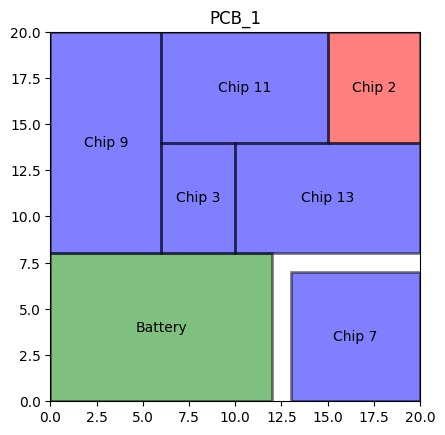
\includegraphics[width=\linewidth]{assets/pcb-1-a.jpeg}
                    \caption{PCB 1, with Camera A}
                    \label{fig:pcb1}
                \end{minipage}\hfill
                \begin{minipage}{0.45\textwidth}
                    \centering
                    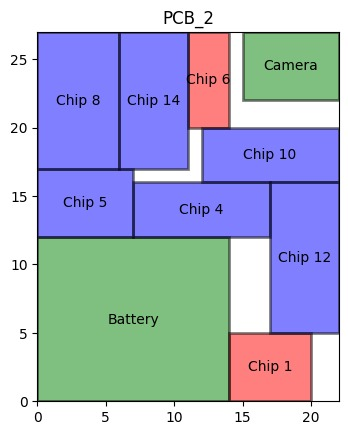
\includegraphics[width=\linewidth]{assets/pcb-2-a.jpeg}
                    \caption{PCB 2, with Camera A}
                    \label{fig:pcb2}
                \end{minipage}
            \end{figure}

            \subsubsection{Visualization Exercise 2b}
            \begin{figure}[H]
                \centering
                \begin{minipage}{0.45\textwidth}
                    \centering
                    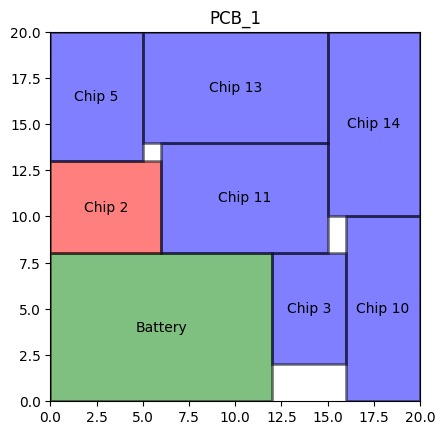
\includegraphics[width=\linewidth]{assets/pcb-1-b.jpeg}
                    \caption{PCB 1, with Camera B}
                    \label{fig:pcb1b}
                \end{minipage}\hfill
                \begin{minipage}{0.45\textwidth}
                    \centering
                    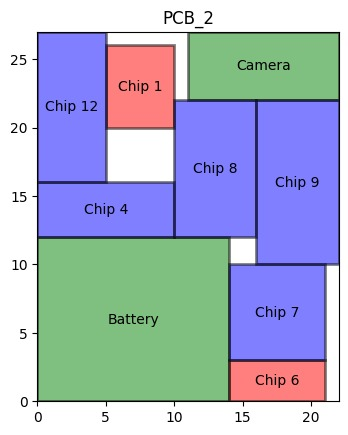
\includegraphics[width=\linewidth]{assets/pcb-2-b.jpeg}
                    \caption{PCB 2, with Camera B}
                    \label{fig:pcb2b}
                \end{minipage}
            \end{figure}

            \subsubsection{Visualization Exercise 2c}

            \begin{itemize}
                \item UNSAT
            \end{itemize}

    \section{Problem 3: Food Supply}
Three villages depend on a truck for food deliveries while consuming food continuously.
Determine how long they can survive with the original truck capacity and whether increasing its capacity allows them to be supplied indefinitely.
	% We dont really need to add the process, and how/what order we implemented it
	% This subsection is just that so I'll just comment it out
	% 
	% \subsection{Approach}
	% 
	% When I started I did not know how I was supposed to solve this. I could
	% not see a way to dynamically run more steps in z3. The trick is to
	% realize you do not need to. You can dynamically build a solver for $1,
	% 2, ... n$ until you find what you're looking for. When I figured that
	% out it wasn't that hard anymore.
	% 
	% I then created a lot of util functions and types to make implementing
	% the assertions easier. When I didn't really knew how to implement the
	% code I went back to the report to instead do it as logic formulas.
	% This was easier to implement then code because of the lack of overhead
	% of those very types.
	% 
	% When the logic was finished in the report, it was then really easy to
	% implement the same assertions as code using those helper types.
    \subsection{Solutions}
        
        \subsubsection{constants}
            \begin{itemize}
                \item truck capacity
                    $\texttt{trucks\_max\_capacity} = \begin{cases}
                        130 & \text{for sub-question a } \\
                        150 & \text{for sub-question b } \\
                    \end{cases}$
                \item The max steps to emulate:
                    \texttt{max\_steps}
            \end{itemize}

        \subsubsection{Variables}
            \begin{itemize}
                \item
                    $\mathit{f}_{s,v} \in \mathbb{Z}$ representing the food left in
                    village $v$, at step $s$.
                \item
                    $\beta_{s} \in \mathbb{Z}$ representing the food in the
                    truck at step $s$.
                \item
                    $\mathit{t}_{s} \in \mathbb{Z}$ representing the total
                    time passed at step $s$.
                \item
                    $\ell_{s,l} \in \mathbb{B}$ representing whether the
                    truck is at location $l$ on step $s$.
            \end{itemize}

        \subsubsection{Sets}
            \begin{itemize}
                \item 
                    The set of villages: $V = \big\{ A, B, C \big\}$.
                \item 
                    The set of supplies: $W = \big\{ S \big\}$.
                \item
                    The set of locations: $L = V \cup W$
                \item
                    The set of routes: $R = \big\{
                        (A, B), (B, A),
                        (A, S), (S, A),
                        (A, C), (C, A),
                        (B, C), (C, B),
                        (C, S), (S, C)
                    \big\}$
                \item
                    The set of steps: $\mathbb{S} = \big\{
                        1, 2, ..., \texttt{ max\_steps}
                    \big\}$
                \item
                    The set of linked steps: $\mathbb{S}_t = \big\{
                        (1, 2), (2, 3), ..., 
                        (\texttt{ max\_steps} - 1,\texttt{ max\_steps})
                    \big\}$
            \end{itemize}

        \subsubsection{Functions}        
            \begin{itemize}
                \item 
                    A function the capacity of a village $v$:
                    \[
                        c : V \to \mathbb{N},\qquad c(v) = \begin{cases}
                            90  & \text{if } v = A \\
                            120 & \text{if } v = B \\
                            90  & \text{if } v = C
                        \end{cases}
                    \]
                \item 
                    A function to get the distance between two locations:
                    \[
                        d : R \to \mathbb{N},\qquad d(r) = \begin{cases}
                            15 & \text{if } r \in \big\{
                                (A, S), (S, A), (C, S), (S, C)
                            \big\} \\
                            17 & \text{if } r \in \big\{
                                (A, B), (B, A)
                            \big\}  \\
                            13 & \text{if } r = (B, C) \\
                            9 & \text{if } r = (C, B) \\
                            12 & \text{if } r \in \big\{
                                (A, C), (C, A)
                            \big\}  \\
                            1 & \text{if } r \in \big\{
                                (S, S), (A, A), (B, B), (C, C)
                            \big\} \\
                        \end{cases}
                    \]
                    note that the distance to the same place is $1$. This is
                    done on purpose. This allows you to "travel" to the same
                    place in $1$ time unit. Effectively allowing you to wait.
            \end{itemize}
    
        \subsubsection{Assertions}
            \begin{itemize}
                \item 
                    Asserting that a village at any step has a valid amount of food:
                    \[
                        \bigwedge_{(s, v) \in \mathbb{S} \times V} \bigg(
                            0 < \mathit{f}_{s,v} \le c(v)
                        \bigg)
                    \]
                \item 
                    Asserting that the truck at any step has a valid amount of food:
                    \[
                        \bigwedge_{s \in \mathbb{S}} \bigg(
                            0 < \beta_{s} \le \texttt{trucks\_max\_capacity}
                        \bigg)
                    \]
                \item 
                    Asserting that the truck must be at exactly one location:
                    \[
                        \bigwedge_{s \in \mathbb{S}} \bigg(
                            1 = \sum_{l \in L} \Big(
                                \operatorname{ite}\big(
                                    \ell_{s,l},\ 1,\ 0
                                \big)
                            \Big)
                        \bigg)
                    \]
                \item 
                    Asserting that you can only travel routes:
                    \[
                        \bigwedge_{\substack{
                            (s_1, s_2) \in \mathbb{S}_t \\
                            (l_1, l_2) \in L \times L
                        }} \bigg(
                            \Big( 
                                    \ell_{s_1,l_1}
                                \wedge
                                    (l_1, l_2) \not \in R
                            \Big) \implies \neg \ell_{s_2,l_2}
                        \bigg)
                    \]
                \item 
                    Asserting that time passes as you travel:
                    \[
                        \bigwedge_{\substack{
                            (s_1, s_2) \in \mathbb{S}_t \\
                            (l_1, l_2) = r \in R
                        }} \bigg(
                            \Big( 
                                \ell_{s_1,l_1} \wedge \ell_{s_2,l_2}
                            \Big) \implies \Big( 
                                \mathit{t}_{s_2} = \mathit{t}_{s_1} + d(r)
                            \Big)
                        \bigg)
                    \]
                \item 
                    Asserting that the truck is refilled at a supply:
                    \[
                        \bigwedge_{\substack{
                            s \in \mathbb{S} \\
                            l \in W
                        }} \bigg(
                            \ell_{s,l} \implies \beta_{s} = \texttt{trucks\_max\_capacity}
                        \bigg)
                    \]
                \item 
                    Asserting that the food goes down as time passes, but if
                    the truck is at that location, that location may refill.
                    \[
                        \bigwedge_{\substack{
                            (s_1,s_2) \in \mathbb{S}_t \\
                            v \in V
                        }}
                        \left(
                            \mathit{f}_{s_2,v}
                            =
                            \mathit{f}_{s_1,v}
                            -
                            \Delta_\mathit{t}
                            +
                            \operatorname{ite}\big(
                                \ell_{s_2,v}, 
                                \Delta_\beta, 
                                0
                            \big)
                        \right)
                        \qquad \text{ where } 
                            \Delta_\mathit{t} = \mathit{t}_{s_2} - \mathit{t}_{s_1}
                            \text{ and }
                            \Delta_\beta = \beta_{s_1} - \beta_{s_2}
                    \]
                \item 
                    Asserting the starting state, all villages are full, and so is the truck:
                    \[
                        \beta_{s} = \texttt{trucks\_max\_capacity}    
                        \wedge 
                        \left(
                            \bigwedge_{\substack{
                                v \in V
                            }} \mathit{f}_{s,v} = c(v)
                        \right)
                        \qquad \text{ where } 
                            s = 0
                    \]
                \item 
                    Asserting that food in the truck can not go up on village tiles:
                    \[
                        \bigwedge_{\substack{
                            (s_1, s_2) \in \mathbb{S}_t \\
                            l \in L
                        }}\left(
                            \ell_{s_2,l} \wedge l \not\in W \implies \beta_{s_2} \le \beta_{s_1}
                        \right)
                    \]
            \end{itemize}

        \noindent For sub-question A we just wish to prove that we cannot keep these
        satisfying all these constraints. So we keep increasing the amount of steps
        until there is no way to satisfy them.

        For sub-question B we also wish to prove that we can keep going
        forever. We are going to do this by proving there is some order of steps
        such that we get to the exact same state again. Proving that we can keep
        going forever. For that we've made the following assertion:
        \[
            \left(
                \bigvee_{\substack{
                    (s_1, s_2) \in \mathbb{S} \times \mathbb{S}
                }}
                % is not the same time
                s_1 \not = s_2 
                % Truck has same amount of food
                \wedge \beta_{s_1} = \beta_{s_2}
                % Truck is in same location
                \wedge \left(
                    \bigwedge_{\substack{
                        l \in L
                    }} \ell_{s_1,l} = \ell_{s_1,l}
                \right)
                % all villages have the same amount of food as before
                \wedge \left(
                    \bigwedge_{\substack{
                        v \in V
                    }} f_{s_1,v} = f_{s_2,v}
                \right)
            \right)
        \]

    \subsection{Results}

        \subsubsection{Visualisation Exercise 3a}
            This was UNSAT.

        \subsubsection{Visualisation Exercise 3b}

            \begin{table}[h]
                \centering
                \label{tab:exercise3b}
                \begin{tabular}{cc|ccccc}
                    \textbf{$s$} & \textbf{$t_s$} & \textbf{$F_{A,s}$} &
                    \textbf{$F_{B,s}$} & \textbf{$F_{C,s}$} & \textbf{$\beta_s$} &
                    \textbf{$\ell_{s,?}$} \\
                    \hline
                    0 & 0   & 60 & 60  & 60 & 150 & S \\
                    1 & 15  & 67 & 45  & 45 & 128 & A \\ \rowcolor{gray!15}
                    2 & 30  & 52 & 30  & 30 & 150 & S \\
                    3 & 45  & 37 & 15  & 16 & 149 & C \\
                    4 & 54  & 28 & 100 & 7  & 55  & B \\
                    5 & 67  & 15 & 87  & 39 & 10  & C \\
                    6 & 82  & 0  & 72  & 24 & 150 & S \\
                    7 & 97  & 79 & 57  & 9  & 56  & A \\
                    8 & 109 & 67 & 45  & 45 & 8   & C \\ \rowcolor{gray!15}
                    9 & 124 & 52 & 30  & 30 & 150 & S \\
                \end{tabular}
                \caption{The steps and the results for 3b proving perpetual looping.}
            \end{table}

    \section{Problem 4: Program Verification}
A C program uses nondeterministic choices to update two variables before checking an assertion.
Determine which values of $k$ can cause the program to crash and provide an execution for each possible crash.

\subsection{Solution}
We identify multiple parameters for the problem
\begin{itemize}
\item $q$ the iteration bound. We set this to the maximum amount the loop would be able to iterate which is 40.
\item $a_i \in \mathbb{N}$ the value of the $a$ variable of the $i$th iteration
\item $b_i \in \mathbb{N}$ the value of the $b$ variable of the $i$th iteration
\item $k \in \{0..10\}$ the constant added to the last \verb|if| statement.
\end{itemize}

The begin of the snippet defines $a$ and $b$ to 1. Which we encode as 
\[
a_0 = 1 \wedge b_0 = 1
\]

Encoding each iterations we have bound it to $q$. Leading to the formula.
\begin{equation} \label{eq:e4-2}
\bigwedge_{1 \le i \le q} F
\end{equation}
where $F$ is the formula of the iteration body.

Since $q$ is the maximum number of iterations not all runs need 40 iterations. Therefore we guard the formula with the condition of the while loop:
\begin{equation}
\big( \  a_{i-1} < 180 \Rightarrow F) \big) \wedge 
\big( \ a_{i-1} \geq 180 \Rightarrow ( b_i = b_{i-1} \wedge a_i = a_{i-1} )\big)
\end{equation}
where $F$ is the formula of the iteration body.

Encoding the case \verb|__nondet__()| returns true we get
\[
(b_i = b_{i-1} + 3 \wedge a_i = a_{i-1} + 2 * b_i )
\]
Encoding the case where \verb|__nondet__()| returns false we get
\[
(b_i = b_{i-1} + a_{i-1} \wedge a_i = a_{i-1} + 5 )
\]

Encoding a \verb|if-then-else| statement normally would result in the form $(c \Rightarrow F_1) \wedge (\neg c \Rightarrow F_2)$.
Since the condition is non deterministic we cannot encode the condition that way, we treat it as either case is correct, therefore we encode it as $F_1 \vee F_2$.
\begin{equation} \label{eq:e4-1}
(b_i = b_{i-1} + 3 \wedge a_i = a_{i-1} + 2 * b_i ) \vee
(b_i = b_{i-1} + a_{i-1} \wedge a_i = a_{i-1} + 5 )
\end{equation}


Normally for program correctness you would prove \texttt{UNSAT} for $\neg Q$.
But in this case we are trying to verify than no trace could lead to the condition resulting in true.
So we would prove \texttt{UNSAT} for $Q$. This results in.
\[
b_q = 190 + k
\]

Combining all the components together we get the formula:
\begin{equation}
\begin{split}
	& a_0 = 1 \wedge b_0 = 1 \\
	& \bigg(\bigwedge_{1 \le i \le q}  \\
		& \quad \big( \  a_{i-1} < 180 \Rightarrow 
			( b_i = b_{i-1} + 3 \wedge a_i = a_{i-1} + 2 * b_i ) \vee
			( b_i = b_{i-1} + a_{i-1} \wedge a_i = a_{i-1} + 5 )
		\big) \wedge \\ 
		& \quad \big( \ a_{i-1} \geq 180 \Rightarrow 
			( b_i = b_{i-1} \wedge a_i = a_{i-1} )
		\big) \\
	& \bigg) \wedge b_q = 190 + k
\end{split}
\end{equation}

The program builds the formula and for each value for $k$ it checks the formula.

\subsection{Results}
For each K the program returns \texttt{SAT}, meaning the program can crash, or \texttt{UNSAT}, meaning the program cannot crash. It takes about 12 seconds to compute all the results.
\begin{table}[H]
\centering
\caption{Result of Satisfiability}
\label{tab:exercise4}
\begin{tabular}{c|l}
	\textbf{K} & \textbf{Result} \\
    \hline
    %%% T | N | P | S | C | D | W
	0  & Program can not crash.  \\
	1  & Program can crash.  \\
	2  & Program can not crash.  \\
	3  & Program can crash.  \\
	4  & Program can not crash.  \\
	5  & Program can crash.  \\
	6  & Program can crash.  \\
	7  & Program can crash.  \\
	8  & Program can not crash.  \\
	9  & Program can not crash.  \\
	10 & Program can not crash.  \\
\end{tabular}
\end{table}
Per \texttt{k} that can crash we show the values of \texttt{a}, \texttt{b}  and what \verb|__nondet__()| returned.
The trace is given until the loop would exit.
The formula would carry the value over across the rest of the iterations. These traces can be seen in the Table~\ref{tab:exercise4-traces}


\begin{table}[htbp]

\begingroup
	\newcommand\header[1]{
	\hline
		\tabletitle{Trace for k = #1} \\
	\hline
		Iter. & $a$  & $b$ & Condition \\
	\hline}
\caption{Traces for exercise 4}
\label{tab:exercise4-traces}
\def\false{ \texttt{False} }
\def\true{\text{True}}
	\def\tabletitle #1{\multicolumn{4}{c}{\cellcolor{black}\color{white}#1}}
\centering
\begin{tabular}{ccc}

	\begin{tabular}[t]{|rrrr|}
	\header{1}
		0 	  & 1         & 1         & - \\
		1 	  & 6         & 2         & \false \\
		2 	  & 16        & 5         & \true \\
		3 	  & 32        & 8         & \true \\
		4 	  & 54        & 11        & \true \\
		5 	  & 59        & 65        & \false\\
		6 	  & 64        & 124       & \false \\
		7 	  & 69        & 188       & \false \\
		8 	  & 451       & 191       & \true \\
		9 	  & 451       & 191       & - \\
		\multicolumn{4}{|c|}{Left out for brevity} \\
	\hline
	\end{tabular}
	&
	\begin{tabular}[t]{|rrrr|}
	\header{3}
		0  	  & 1    & 1   & -\\
		1  	  & 6    & 2   & \false \\
		2  	  & 11   & 8   & \false \\
		3  	  & 16   & 19  & \false \\
		4  	  & 21   & 35  & \false \\
		5  	  & 26   & 56  & \false \\
		6  	  & 31   & 82  & \false \\
		7  	  & 36   & 113 & \false \\
		8  	  & 41   & 149 & \false \\
		9  	  & 46   & 190 & \false \\
		10 	  & 432  & 193 & \true \\
		11 	  & 432  & 193 & - \\
		\multicolumn{4}{|c|}{Left out for brevity} \\
	\hline
	\end{tabular}
	&
	\begin{tabular}[t]{|rrrr|}
	\header{5}
		0  	  & 1   & 1    & -\\
		1  	  & 9   & 4    & \true \\
		2  	  & 14  & 13   & \false \\
		3  	  & 46  & 16   & \true \\
		4  	  & 84  & 19   & \true \\
		5  	  & 89  & 103  & \false \\
		6  	  & 94  & 192  & \false \\
		7  	  & 484 & 195  & \true \\
		8  	  & 484 & 195  & - \\
		\multicolumn{4}{|c|}{Left out for brevity} \\
	\hline
	\end{tabular}
	\\ 
	\begin{tabular}[t]{|rrrr|}
	\header{6}
		0  	  & 1   & 1    & -\\
		1  	  & 9   & 4    & \true \\
		2  	  & 14  & 13   & \false \\
		3  	  & 19  & 27   & \false \\
		4  	  & 79  & 30   & \true \\
		5  	  & 84  & 109  & \false \\
		6  	  & 89  & 193  & \false \\
		7  	  & 481 & 196  & \true \\
		8  	  & 481 & 196  & - \\
		\multicolumn{4}{|c|}{Left out for brevity} \\
	\hline
	\end{tabular}

	&

	\begin{tabular}[t]{|rrrr|}
	\header{7}
		0  	  & 1 & 1      & -\\
		1  	  & 6 & 2      & \false \\
		2  	  & 11 & 8     & \false \\
		3  	  & 16 & 19    & \false \\
		4  	  & 60 & 22    & \true \\
		5  	  & 110 & 25   & \true \\
		6  	  & 166 & 28   & \true \\
		7  	  & 171 & 194  & \false \\
		8  	  & 565 & 197  & \true \\
		9  	  & 565 & 197  & - \\
		\multicolumn{4}{|c|}{Left out for brevity} \\
	\hline
	\end{tabular}
	&\\
\end{tabular}
\endgroup
\end{table}

\subsection{Remarks}
For the formula we have bound $q$ to be 40, which is the maximum amount of iterations the loop would be able to make. This does lead to the formula to maybe bigger than it needs.

    \section{Configurable Systems}
We are given a configuration system, and we need to reason about the configurations that contain the least amount of selected features.


\begingroup
\newcommand\fn[2]{\mathtt{#1}(#2)}
\newcommand\hi[1]{\fn{dec}{#1, 1}}
\newcommand\lo[1]{\fn{dec}{#1, 0}}



\subsection{Solution}
We identify the following parameters of the problem:
\begin{itemize}
  \item $n \in \mathbb{N}$ is the number of features, given in the header of the DIMACS file.
  \item $\varphi$ is the CNF formula from the DIMACS file. It consists of clauses $C_1,\dots,C_m$, and every clause is a set of literals over the features.
  \item $S=\{x_{218},x_{311}\}$ is the set of essential features.
\end{itemize}
We introduce the following variables:
\begin{itemize}
  \item $x_i \in \mathbb{B}$ for $i=1,\dots,n$: the value of $x_i$ is true if and only if feature $i$ is selected. The BDD variable order is given in the DIMACS file
  \item $\mathit{var}(u)$ and $\mathit{level}(u)\in\{1,\dots,n+1\}$ are the variable and the level of a BDD node $u$, so $\mathit{level}(x_i)=i$. The terminals $\top$ and $\bot$ are at level $n+1$. The children of $u$ are $\hi{u}$ and $\lo{u}$.
  \item $\mathtt{min\_cost}(u)\in\mathbb{N}\cup\{\infty\}$ is the smallest number of true variables on a path from $u$ to $\top$.
\end{itemize}

\subsubsection{Building the BDD}
We are given a DIMACS file, which contains an CNF.
We parse the CNF and after that we can build the BDD by iterating over the clauses, combining the variables with $\vee$ and combining the clauses with $\wedge$. 

\subsubsection{Computing the minimum amount of variables needed}
To compute the minimum amount of work we can 'walk' through the BDD, working from an bottoms-up manner we count the amount of 'true' edges we see.
This can be formulised in the function
\[
\fn{min\_cost}{n} =
\begin{cases}
\infty, & n = \bot \\
0, & n = \top \\
\min\bigl( \fn{min\_cost}{\lo{n}}, 1 + \fn{min\_cost}{\hi{n}} \bigr) & otherwise
\end{cases}
\]


\subsubsection{Computing the minimum amount of variables needed with essential variables}
Certain variables can be deemed as essentials. Those variables \textit{must} be true.
We achieve that though using the already build BDD and asserting those essential formulas.
The essential variables are: $\{x_{218}, x_{311}\}$. This produces the BDD:
\[
F \wedge x_{218} \wedge x_{311}
\]
Where $F$ is the BDD given in the DIMACS file.

\subsubsection{Building the BDD for the function with the minimum amount}
We again 'walk' through the BDD, but instead of computing a simple statistics we now produce a new BDD.
We do this via the \verb|min_config| function
\[
\fn{min\_config}{n} =
\begin{cases}
\bot & n = \bot \\
\top & n = \top \\
(\fn{var}{n} \wedge \fn{min\_hi}{n,\hi{n}}) \vee (\neg \fn{var}{n} \wedge \fn{min\_lo}{n,\lo{n}}) & otherwise
\end{cases}
\]
\[
\fn{min\_hi}{n, m} =
\begin{cases}
\bot & \fn{min\_cost}{m} \ge \fn{min\_cost}{n} \\
\fn{min\_config}{m} \wedge \fn{skip}{n,m}  & otherwise
\end{cases}
\]
\[
\fn{min\_lo}{n, m} =
\begin{cases}
\bot & \fn{min\_cost}{m} > \fn{min\_cost}{n} \\
\fn{min\_config}{m} \wedge \fn{skip}{n,m}  & otherwise
\end{cases}
\]
\[
  \fn{skip}{u,w} =\bigwedge_{\mathit{level}(u) < i < \mathit{level}(w)} \neg x_i 
\]

After we have restricted the BDD to only the configurations with the minimum amount, we also need to constrict the variables that may have been removed from the BDD.
We do this by collecting all the used variables in the BDD and asserting them all to false.
\[
\fn{used\_vars}{n} =
\begin{cases}
\emptyset & n = \bot \vee n = \top \\
\{\fn{var}{n}\} \cup \fn{used\_vars}{\hi{n}} \cup \fn{used\_vars}{\lo{n}} & otherwise
\end{cases}
\]
\[
\fn{constrict\_to\_used\_vars}{n,vars} = n \bigwedge_{v \in vars\backslash \fn{used\_vars}{n}} \neg v
\]


\subsubsection{Verifying SAT count for restricted BDD function}
To add an extra verification step we add a \verb|minimum_count| function that counts amount of SAT count with respect to the constraints the same as \verb|min_hi| and \verb|min_lo|. An important distinction is it only counts the paths that lead to a $\top$, it does not account for unused variables and skipped levels.
\[
\fn{minimum\_count}{n} = 
\begin{cases}
0 & n = \bot \\
1 & n = \top \\
\fn{count\_lo}{n,\lo{n}} + \fn{count\_hi}{n,\hi{n}} & otherwise\\
\end{cases}
\]
\[
\fn{count\_lo}{n,m} =
\begin{cases}
0 & \fn{min\_cost}{m} > \fn{min\_cost}{n} \\
\fn{minimum\_count}{m} & otherwise\\
\end{cases}
\]
\[
\fn{count\_hi}{n,m} = 
\begin{cases}
0 & \fn{min\_cost}{m} \ge \fn{min\_cost}{n} \\
\fn{minimum\_count}{m} & otherwise\\
\end{cases}
\]

\subsubsection{Runtime}
Each of the function that work on a BDD in its given form would visit every node once and take $O(|BDD|)$. We can reduce that by introducing caches for the BDDFunctions.
Each function that is presented contains a cache. If the given BDDFunction is already in the cache that result is returned, if not it is computed and added in the cache.
The function \verb|minimum_count|, \verb|min_config| and their respective sub functions use two caches.
The first one is the cache for the actual computation, the second cache is the \textit{cost\_cache}, that is passed to the \verb|min_cost| function.
Since the \verb|min_cost| function walks through the BDD populating the \textit{cost\_cache}, all of the sub functions in \verb|minimum_count| and \verb|min_config| use the already populated \textit{cost\_cache}.
Meaning that the those \verb|min_cost| function calls amounts to only a cache lookup.


\subsection{Results}
Per given DIMACS file we provide the calculated result in Table~\ref{tab:exercise-5-res}
\def\tabletitle #1{\multicolumn{2}{c}{\cellcolor{black}\color{white}#1}}
\newcommand\resulttable[9]{
	\begin{tabular}[t]{lp{8.5cm}}
		\tabletitle{Result for #1} \\
		(i) BDD nodes of $\llbracket \varphi \rrbracket$ & #3 \\
		(ii) Valid configurations $|V|$ & \texttt{\seqsplit{#4}} \\
		(iii) $|F\upharpoonright_{cmin}|$ & #5 \\
		(iv) Essential $|F\upharpoonright_{cmin}|$ for $S=\{x_{218},x_{311}\}$ & #6 \\
		(v) BDD nodes of $\llbracket \varphi \rrbracket_{cmin}$ & #7 \\
		(vi) Number of minimum configurations & #8 \\
		Time to run & #9 \\
\bottomrule
\end{tabular}
}
 
\begin{table}[htbp]
\caption{Results}
\centering
\begin{tabular}{c}
	\resulttable{buildroot}{565}{1000}{197929412613795104033186650529764251995382268085040059140299644922581611052953218858293468858114370125417172798513453704215828256540658252191740135040064962560}{1}{14}{567}{1}{$\sim$0.7s}
	\\
	\resulttable{busybox}{820}{3076}{341966771173357574203468511726402787658846470020778853449916660355015748144503172810981395757363854768801367747323733822923115327180062924636321384290977279599243935937986560000000000000000000000}{17}{24}{847}{243}{$\sim$1.5s}
	\\
	\resulttable{embtoolkit}{2108}{172157}{5269086459380001633643953865313843951587769385459462783768187763744059253901124797424957712252293478301274200994406811283718331120294266116775137066700763565336063060585502617122754794227972693181096959562137510764573788550603417290201944648467575812000557794560479278383157151334042379118437642922099801799434308519509535427929029197430784}{50}{111}{3441}{102114}{$\sim$2m 20s}
	\\
	\resulttable{toybox}{544}{949}{144991790900969472}{28}{51}{610}{192}{$\sim$0.6s}
	\\
	\resulttable{uClinux}{1850}{2667}{16296287810675888690147565507275025288411747149327490005089123594835050398106693649467179008}{7}{11}{1852}{1}{$\sim$5.4s}

	\label{tab:exercise-5-res}
\end{tabular}
\end{table}

\endgroup

    \section{Exercise 6}

    In this exercise, we analyze directed graphs using Binary Decision Diagrams
    (BDDs). These graphs are obtained from social networks extracted from Pokec
    (a Slovakian social network) and Twitter. All nodes within these directed
    graphs are labeled with $0$ or $1$. The total number of nodes and
    transitions is stated in the table below:

    $$ 
    \begin{array}{lcc} \hline \textbf{Graph} & \textbf{\#Nodes} &
        \textbf{\# Transitions} \\ \hline 
    \text{Pokec Small} & 99999 & 1768496 \\ 
    \text{Pokec Medium} & 499999 & 13225726\\ 
    \text{Pokec} & 1632803 & 30622564 \\ 
    \text{Twitter Congress} &  475 & 13289 \\ \hline 
    \end{array}
    $$

    To analyze these graphs we require three specific BDDs, namely:

    \begin{itemize}
        \item A BDD that represents the nodes with label $0$
        \item A BDD that represents the nodes with label $1$
        \item A BDD that represents the transitions from a source node to a
            target node
    \end{itemize}

    \subsection{Results:}
        
        \subsubsection{Exercise A:}
            We construct the BDDs as follows:

            \begin{itemize}
                \item Let $N$ be the set of nodes.
                \item Let $T$ be the set of transitions.
                \item Let $S$ be the number of nodes.
                \item Let $l$ be the length of the encoding calculated by:
                \[
                l = \lceil \log_2(S) \rceil
                \]
            \end{itemize}

            \begin{itemize}
                \item Let $L(n)$ be the $0/1$-label for node $n$.
                \item Let $\text{enc}(n)$ be an encoding function that encodes
                    the identifier for node $n$ to $l$ number of bits.
                \item Let $\text{source}(t)$ be the source node of transition
                    $t$.
                \item Let $\text{target}(t)$ be the target node of transition
                    $t$.
            \end{itemize}

            Below are the three BDD's constructed by their corresponding CNF
            formulas:

            \begin{itemize}
                \item $BDD_0 :$
                \[
                    \bigvee_{n \in S \land L(n) = 0} \bigwedge_{x \in enc(n)}x
                \]
                \item $BDD_1 :$
                \[
                    \bigvee_{n \in S \land L(n) = 1} \bigwedge_{x \in enc(n)}x
                \]
                \item $BDD_T :$
                \[
                    \bigvee_{t \in T}( (\bigwedge_{x \in enc(source(t))}x )
                    \land(\bigwedge_{x' \in enc(target(t))}x'))
                \]
            \end{itemize}

            Resulting in BDDs with the following number of nodes:

            \begin{table}[h]
                \centering
                \begin{tabular}{l c c c c}
                    \toprule
                    & Pokec Small & Pokec Medium & Pokec & Twitter Congress \\
                    \midrule
                    $BDD_0$ & 12271 & 52746 & 137785 & 9 \\
                    $BDD_1$ & 12271 & 52747 & 137787 & 17 \\
                    $BDD_T$ & 3560 & 11211 & 59438 & 37 \\
                    \bottomrule
                \end{tabular}
            \end{table}

            With these BDDs, we can look up a specific node label or determine
            whether a transition exists in $O(l)$ time. Having these three BDDs
            to represent the direct graph allows us to analyze these graphs in
            the following two exercises.

        \subsubsection{Exercises B \& C:}

            For exercise $B$, we find the number of reachable nodes, and for
            exercise $C$, we find the number of reachable nodes along an
            $0/1$-alternating path. For both, we use the node with ID $1$ as
            the starting node. The table below reports our results for all
            graphs with their running times.

            \begin{table}[h]
                \centering
                \vspace{0.25cm}
                \begin{tabular}{l c c c c}
                    \toprule
                    \textbf{Metric} & \textbf{Pokec Small} &
                    \textbf{Pokec Medium} & \textbf{Pokec} &
                    \textbf{Twitter Congress} \\
                    \midrule
                    \#Nodes & 
                    99999 & 499999 & 1632803 & 475 \\
                    \#Transitions & 
                    1768496 & 13225726 & 30622564 & 13289 \\
                    \#Nodes Reachable from $1$ & 
                    99998 & 499998 & 1632802 & 474 \\
                    Running Time &
                    1.205781 s & 13.080146 s & 32.543689 s & 0.006385 s \\
                    \addlinespace
                    \#Nodes Reachable by a $0/1$-Path &
                    42026 & 197222 & 552525 & 383 \\
                    Running Time & 
                    3.519633 s & 22.104163 s & 82.379408 s & 0.008883 s \\
                    \bottomrule
                \end{tabular}
            \end{table}

    \section{Formula 1 Tracks}
\textbf{Note: this section is a work in progress.}

\texttt{SAT City} has been asked to host a race in the new Formula~1 season.
The mayor has tasked you with finding an optimal circuit through the city,
subject to the following requirements:
\begin{itemize}
  \item The circuit must use existing roads only, no roads may be built and no buildings destroyed.
  \item The circuit must visit at least $m$ of the $n$ points of interest in the city.
  \item The length of the circuit must be between $\ell_{\min}$ and $\ell_{\max}$.
  \item To prevent injuries, the circuit may never cross itself.
  \item The circuit must contain between $c_{\min}$ and $c_{\max}$ corners.
  \item As the cars race 50 laps, the start and end location must coincide, i.e.\ the circuit is a single closed loop.
  \item Some roads require renovation before the race may use them, due to time at most $3$ roads may be renovated.
  \item The total cost of the race (permits and renovations) must be minimized.
\end{itemize}
The mayor has provided a overview of all the roads.
He has been kind enough to color the points of interests in blue, 
and colored the roads that would need to be renovated to red.
\begin{figure}
\centering
\caption{Layout of \texttt{SAT City}}
\newcommand{\baseunit}{50}   % metres per grid square
\newcommand{\gs}{0.8}        % drawing scale: cm per grid square
% =========================================

\begin{tikzpicture}[x=0.8 cm,y=0.8 cm,
  v/.style={circle,fill,inner sep=1.4pt},
  I/.style={circle,fill,blue,inner sep=1.4pt},
  line/.style={thick,black!60!black},
  line-broken/.style={thick,red!100!black},
  lbl/.style={fill=white,inner sep=1pt,font=\tiny}]

% \edge[style]{start}{end}: draws the segment and labels its length in metres
\newcommand{\edge}[3][line]{\edgeA[#1]#2#3}
\def\edgeA[#1](#2,#3)(#4,#5){%
  \pgfmathparse{veclen((#4)-(#2),(#5)-(#3))*\baseunit}%
  \let\elen\pgfmathresult
  \draw[#1] (#2,#3) -- (#4,#5)
    node[midway,lbl] {\pgfmathprintnumber[fixed,precision=0]{\elen}};}
\newcommand{\bedge}[2]{\edge[line-broken]{#1}{#2}}

% ---- outer frame ----
\edge{(0,0)}{(2,0)}   \edge{(2,0)}{(4,0)}   \edge{(4,0)}{(6,0)}
\edge{(0,0)}{(0,-2)}  \edge{(0,-2)}{(0,-4)} \bedge{(0,-4)}{(0,-5)}
\edge{(0,-5)}{(0,-7)} \edge{(0,-7)}{(0,-10)}
\edge{(0,-10)}{(3,-10)} \edge{(3,-10)}{(5,-10)}
\edge{(6,0)}{(6,-2)}  \edge{(6,-2)}{(6,-4)} \edge{(6,-4)}{(6,-7)} \edge{(6,-7)}{(6,-8)}

% ---- top / upper middle ----
\edge{(4,0)}{(4,-0.5)} \bedge{(4,-0.5)}{(4,-3)}
\edge{(4,-3)}{(4,-5)}  \edge{(4,-5)}{(4,-6)}
\edge{(2,0)}{(2,-1)}   \edge{(2,-1)}{(2,-3)}  \edge{(2,-3)}{(2,-4)}
\edge{(3,-0.5)}{(4,-0.5)} \edge{(4,-0.5)}{(5,-0.5)} \edge{(5,-0.5)}{(6,-2)}
\edge{(3,-0.5)}{(3,-3)} \edge{(3,-3)}{(3,-4)}
\edge{(3,-0.5)}{(2,-3)}
\edge{(3,-3)}{(4,-3)} \edge{(4,-3)}{(5,-3)} \edge{(5,-3)}{(5,-4)}
\edge{(5,-4)}{(6,-4)} \edge{(6,-4)}{(7,-4)}
\edge{(3,-4)}{(2,-4)} \edge{(2,-4)}{(0,-4)}

% ---- upper left ----
\edge{(1,-1)}{(2,-1)}
\edge{(1,-1)}{(1,-2)} \edge{(1,-2)}{(1,-3)} \edge{(1,-3)}{(2,-3)}
\edge{(0,-2)}{(1,-2)}
\edge{(1,-3)}{(0,-4)}

% ---- right side ----
\edge{(6,-2)}{(8,-2)}
\edge{(8,-2)}{(8,-6)} \edge{(8,-6)}{(8,-7)}
\edge{(6,-4)}{(7,-6)}
\edge{(7,-4)}{(7,-6)} \edge{(7,-6)}{(7,-7)}
\bedge{(7,-6)}{(8,-6)}
\edge{(6,-7)}{(7,-7)} \bedge{(7,-7)}{(8,-7)}
\edge{(8,-7)}{(9,-8)} \edge{(9,-8)}{(9,-10)} \edge{(9,-10)}{(8,-11)}
\edge{(8,-11)}{(7,-12)} \edge{(7,-12)}{(4,-12)}
\edge{(8,-7)}{(8,-9)} \edge{(8,-9)}{(7,-10)} \edge{(7,-10)}{(8,-11)}
\edge{(7,-10)}{(7,-12)}
\edge{(7,-10)}{(5,-9)} \edge{(5,-9)}{(2,-9)}
\bedge{(5,-9)}{(5,-10)}

% ---- centre ----
\edge{(2,-5)}{(4,-5)}
\edge{(2,-5)}{(2,-7)} \edge{(2,-7)}{(2,-9)}
\bedge{(2,-7)}{(4,-7)}
\edge{(4,-7)}{(5,-7)} \edge{(5,-7)}{(6,-7)}
\edge{(4,-6)}{(5,-6)} \edge{(5,-6)}{(6,-7)}
\edge{(5,-6)}{(5,-7)} \edge{(5,-7)}{(5,-8)}
\edge{(4,-7)}{(4,-8)} \edge{(4,-8)}{(5,-8)} \edge{(5,-8)}{(6,-8)}
\edge{(4,-7)}{(5,-8)}

% ---- left middle ----
\edge{(0,-5)}{(0.5,-5)} \edge{(0.5,-5)}{(1,-5)}
\edge{(1,-5)}{(1,-6)} \edge{(1,-6)}{(0.5,-6)} \edge{(0.5,-6)}{(0.5,-5)}
\edge{(1,-6)}{(0,-7)} \edge{(0,-7)}{(1,-7)} \edge{(1,-7)}{(1,-6)}
\edge{(0,-7)}{(1,-8)} \edge{(1,-8)}{(0,-10)}

% ---- bottom ----
\edge{(3,-10)}{(3,-11)} \edge{(3,-11)}{(3,-12)}
\edge{(3,-12)}{(2,-12)} \edge{(2,-12)}{(2,-11)} \edge{(2,-11)}{(3,-12)}
\edge{(3,-10)}{(4,-11)} \edge{(4,-11)}{(5,-10)}
\edge{(4,-11)}{(4,-12)}
\edge{(0,-10)}{(1,-11)} \edge{(1,-11)}{(2,-12)}
\edge{(3,-12)}{(4,-12)}

% ---- vertices ----
\foreach \p in {(0,0),(2,0),(4,0),(6,0),(4,-0.5),
  (3,-0.5),(5,-0.5),(1,-1),(2,-1),
  (0,-2),(1,-2),(6,-2),(8,-2),
  (1,-3),(2,-3),(3,-3),(4,-3),(5,-3),
  (0,-4),(2,-4),(3,-4),(5,-4),(6,-4),(7,-4),
  (0,-5),(0.5,-5),(1,-5),(2,-5),(4,-5),(0.5,-6),(1,-6),
  (4,-6),(5,-6),(7,-6),(8,-6),
  (0,-7),(1,-7),(2,-7),(4,-7),(5,-7),(6,-7),(7,-7),(8,-7),
  (1,-8),(4,-8),(5,-8),(6,-8),(9,-8),
  (2,-9),(5,-9),(8,-9),
  (0,-10),(3,-10),(5,-10),(7,-10),(9,-10),
  (1,-11),(2,-11),(3,-11),(4,-11),(8,-11),
  (2,-12),(3,-12),(4,-12),(7,-12)}
  \node[v] at \p {};

% ---- "I" labels ----
\node[I] at (6,0)   {};
\node[I] at (1,-1)  {};
\node[I] at (5,-3)  {};
\node[I] at (7,-4)  {};
\node[I] at (0,-7) {};
\node[I] at (2,-7)  {};
\node[I] at (5,-10)   {};
\node[I] at (9,-10) {};
\node[I] at (3,-12) {};
\end{tikzpicture}
\end{figure}

\subsection{Solution}

\begingroup

\newcommand\ite[3]{\mathtt{ite}(#1,#2,#3)}
We identify the following parameters of the problem:
\begin{itemize}
  \item $m = 4$ is the minimum number of points of interest the track visits.
  \item $n = 6$ is the total number of points of interest in the city.
  \item $a = 7$ is the minimum number of corners.
  \item $b = 24$ is the maximum number of corners.
  \item $l = 1500$\,m is the minimum length of the track.
  \item $k = 6000$\,m is the maximum length of the track.
  \item $\delta_e \in \mathbb{N}$ is the length of road $e$.
  \item $pc_b \in \mathbb{N}$ is the permit cost of block $b$.
\end{itemize}

We use the following sets:
\begin{itemize}
  \item $V$ is the set of intersections and $E$ is the set of roads.
  \item $B$ is the set of street blocks.
  \item $E_b$ is the set of roads adjacent to block $b$.
  \item $E_v$ is the set of roads adjacent to intersection $v$.
  \item $R \subseteq E$ is the set of roads that need to be renovated.
\end{itemize}

To construct the track, we introduce the following variables:
\begin{itemize}
  \item $\alpha_e \in \mathbb{B}$ for $e \in E$: true iff road $e$ is part of the track.
  \item $\beta_{e,e'} \in \mathbb{B}$ for $e,e' \in E$: true iff the roads $e$ and $e'$ contain a point of interest.
  \item $\gamma_{e,e'} \in \mathbb{B}$ for $e,e' \in E$: true iff there is a corner between $e$ and $e'$.
  \item $p_b \in \mathbb{B}$ for $b \in B$: true iff the permit for block $b$ must be paid.
\end{itemize}


\paragraph{Cross.}
The track does not cross it self, that is each intersection has either 0 or 2 roads on the track.
For every intersection $v$ this is expressed by
\[
(\sum_{e \in E_v} \ite{\alpha_e}{1}{0} = 0 \vee \sum_{e \in V_e} \ite{\alpha_e}{1}{0} = 2)
\]

\paragraph{Points of interest.}
The track visits at least $m$ points of interest
\[
\sum_{(e,e') \in E \times E}(\ite{\alpha_{e} \wedge \alpha_{e'} \wedge \beta_{e,e'}}{1}{0}) \ge m
\]

\paragraph{Corners.}
There are between $a$ and $b$ corners
\[
a \leq \sum_{(e,e') \in E \times E} \ite{\alpha_{e} \wedge \alpha_{e'} \wedge \gamma_{e,e'}}{1}{0}) \leq b
\]

\paragraph{Renovations.}
There track requires at most $3$ roads to be renovated
\[
\sum_{e\in R } \ite{\alpha_{e} }{1}{0}) \leq 3
\]

\paragraph{Length.}
The track length is between $k$ and $l$
\[
k \leq \sum_{e \in E} \ite{\alpha_{e} }{\delta_{e}}{0} \leq l
\]

\paragraph{Permits.}
A block needs a permit if an adjacent road is part of the track.
For every block $B$ this is expressed by
\[
  \bigwedge_{e \in E_B} (\alpha_e \Rightarrow p_B).
\]

\paragraph{Objective.}
We minimize the cost of the permits and the renovations (10 per metre):
\[
 \text{minimize} \quad
 \big( \sum_{b \in B} \ite{p_b}{pc_b}{0} \big) + 
 \big( \sum_{e \in R} \ite{\alpha_e}{10 \cdot \delta_e}{0}\big)
\]



\subsection{Result}

\endgroup

    \begin{thebibliography}{9}
\end{thebibliography}

    \appendix


\end{document}
